\documentclass[a4paper,11pt]{article}
\usepackage{amssymb}
\usepackage{geometry}
\usepackage{amsmath}
\usepackage{graphicx}
\usepackage{hyperref}
\hypersetup{colorlinks = true}
\geometry{left=25mm,right=25mm,%
bindingoffset=0mm, top=20mm,bottom=20mm}
\renewcommand{\baselinestretch}{1}
\usepackage{multicol}
\usepackage{indentfirst}
\usepackage{dirtytalk}

\title{Report on Bremorse visualization} 
\author{}
\date{06 January 2021}

\begin{document}

\maketitle

\section{Results}

In \autoref{fig:my_label}, it is found that most of the opinions that think Britain was right to leave the EU has changed over the time. Although there were several spikes and plummets in between the period of July 2016 to July 2018, \autoref{fig:my_label} displays that there have been a gradual decline. As lesser people think it is right for Britain to leave the EU, more comes to agree that it is wrong of her to leave. 

\begin{figure}[h]
    \centering
    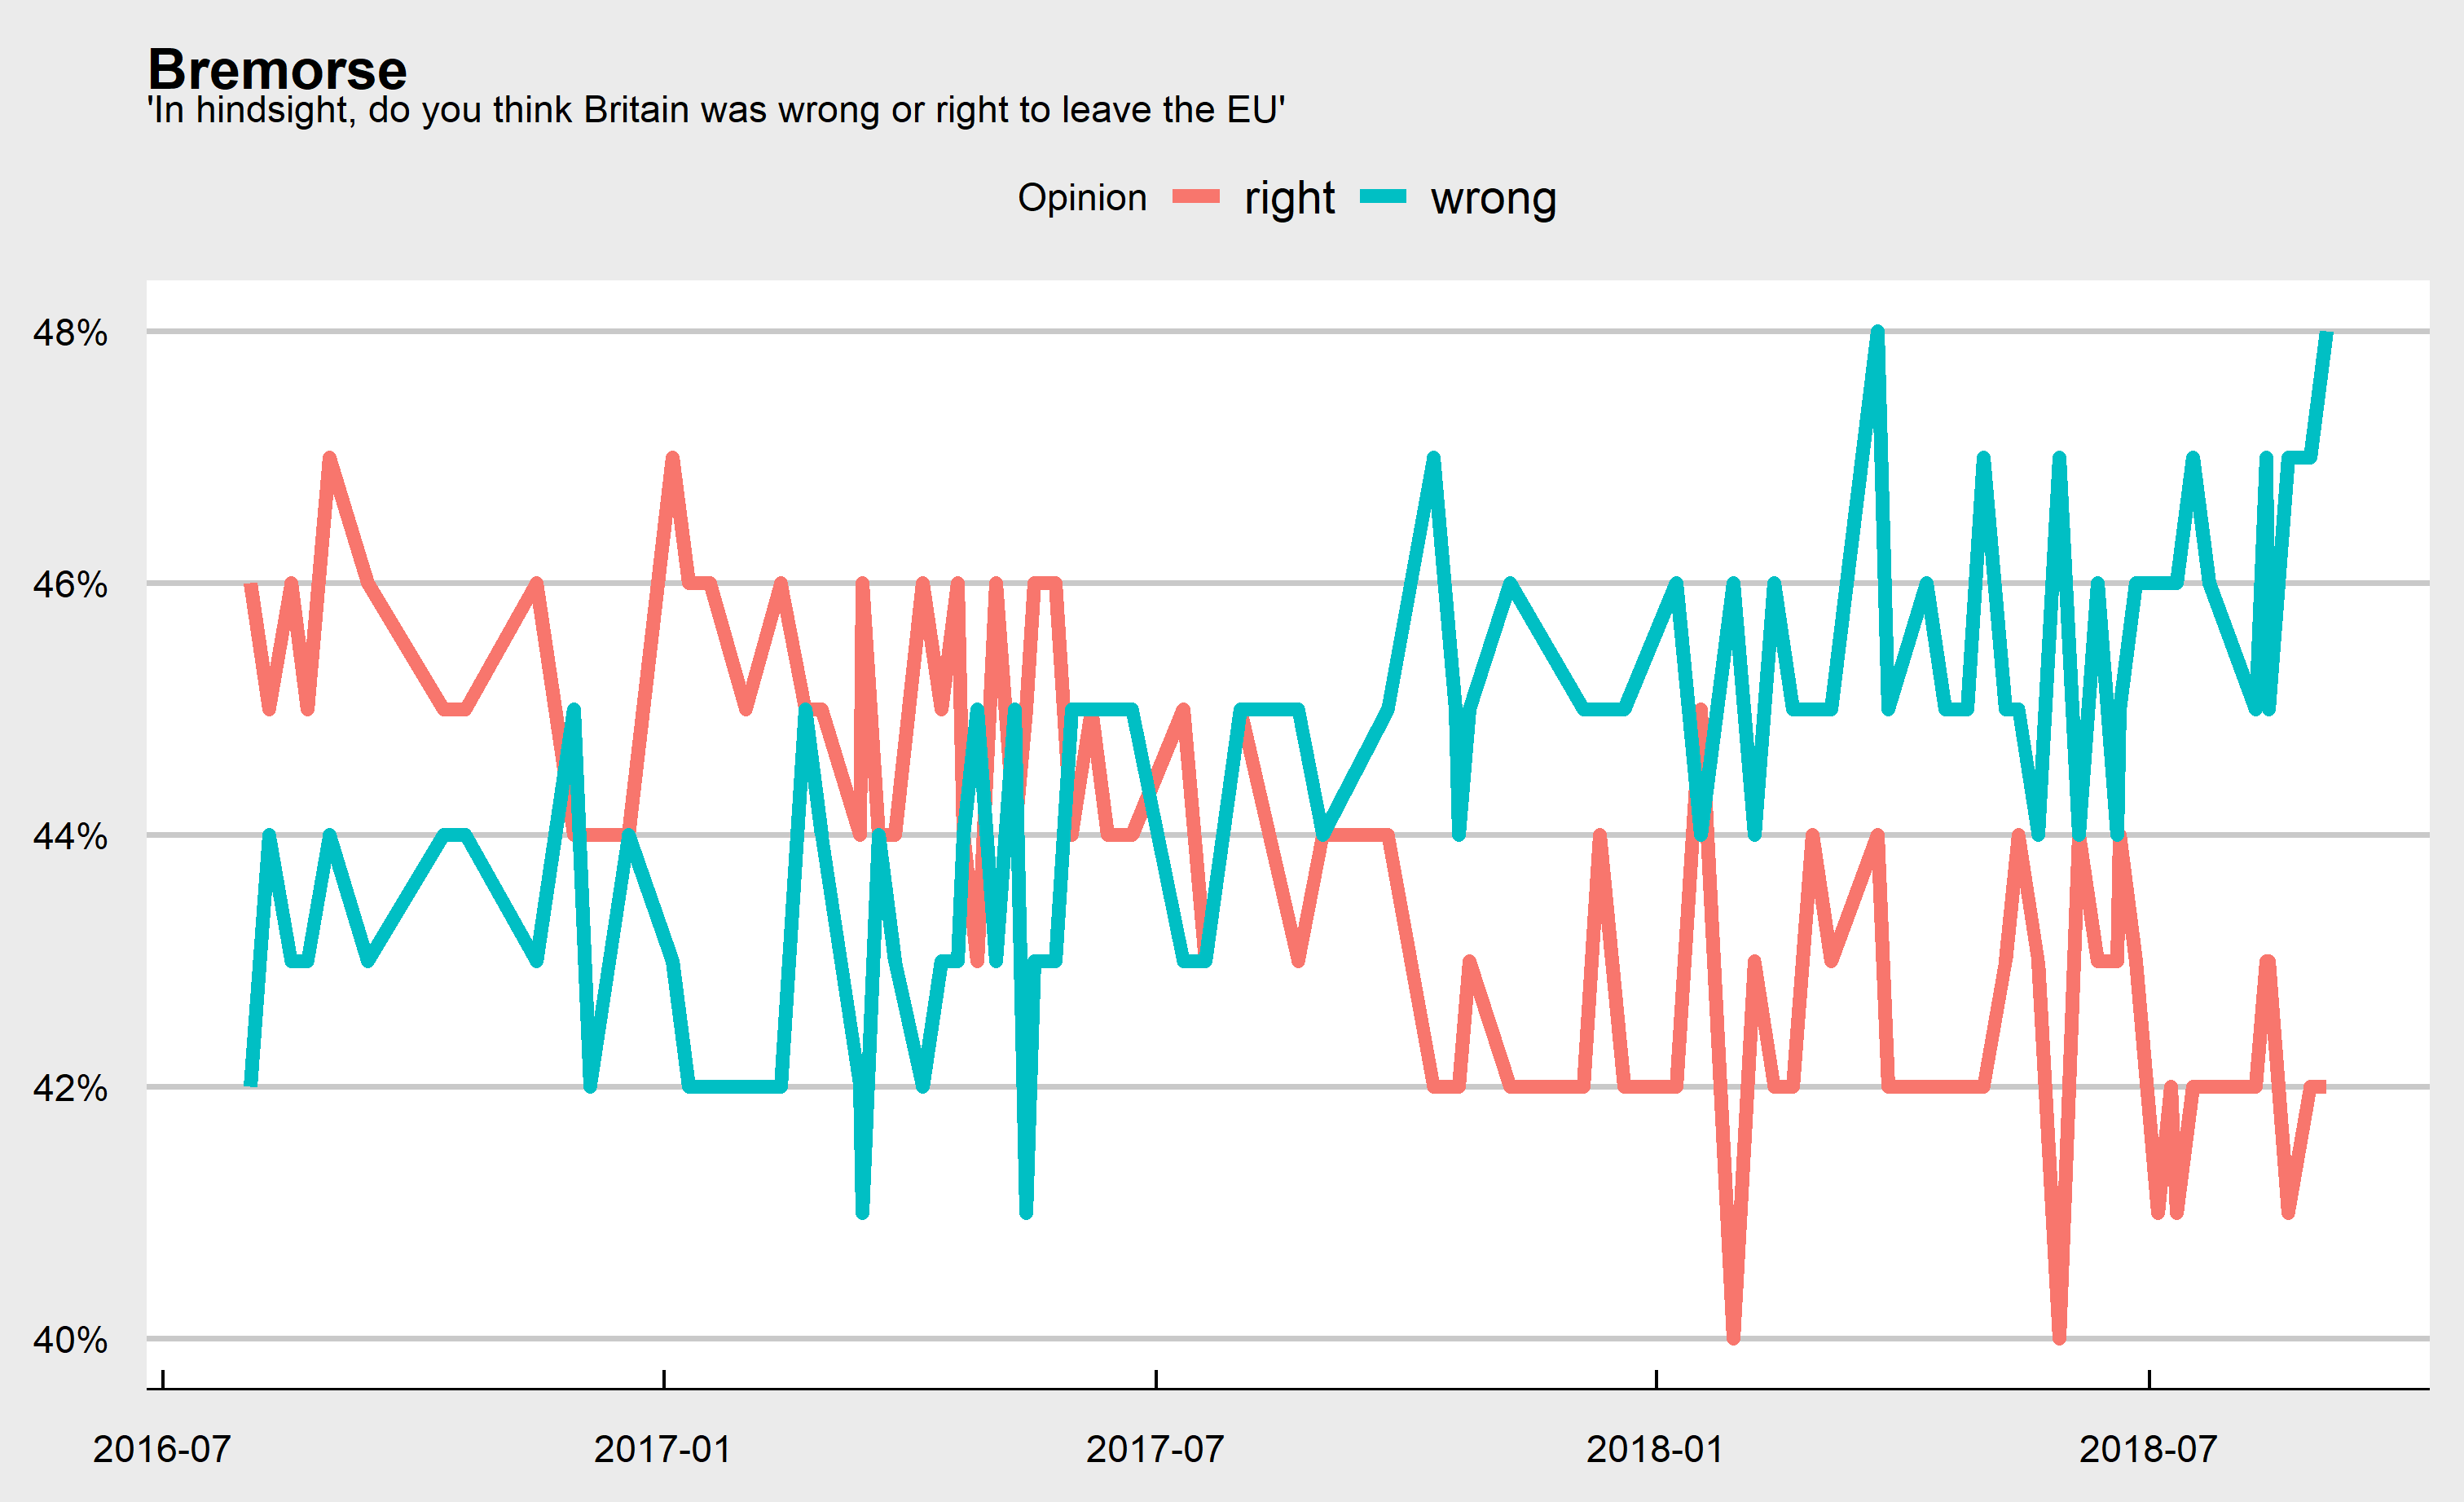
\includegraphics[width = \textwidth]{Bremorse_graph.png}
    \caption{\emph{The Economist's} Bremorse visualization}
    \label{fig:my_label}
\end{figure}

\section{Discussion}
When looking at \autoref{fig:my_label}, there has been fewer people thinking that it is right for Britain. When this dataset was collect, the majority of the people still thinks that it is right. The reason for that would be that during mid-2016 to mid-2017, Britain is at her highest development. As most of the residents in Britain would have felt that the other countries in the EU is bringing down the development of Britain, most agree to her decision in leaving the EU. However, as the year progress after mid-2017 to mid -2018, a lot of people start to change their opinion. For the EU shares information amongst each country, the collective information made the country develops a lot more faster than how Britain would have when she stands alone. Due those development, more people starts to disagree on her decision. The pattern in \autoref{fig:my_label} generally shows that a lot of people are dissatisfied by her decision. However, when looking closely, there have been a few spikes in between January 2018 to July 2018 where some people again agree to her decision to leave. Although there have been a few spikes in between mid-2017 to mid-2018, it can still be seen that the trend for the people who think it is right is declining. 

\section{Conclusion}
Initially, a lot of people have thought that Britain has done the right choice by leaving the EU. However, as the time passes, not many thought it is a right decision after all.  


\end{document}
